% hoot.tex

% Author: Dustin Bachrach, Christopher Nunu, Dan Wallach, Matt Wright

% Revisions:  28 March 2011

\documentclass{sig-alternate}
%\documentclass{acm_proc_article-sp}

\usepackage{amsmath}
\usepackage{times}
\usepackage{mathptm}
\usepackage[scaled=0.87]{helvet} % better visual match w/ Times
\usepackage{graphicx}
\usepackage{balance}
\usepackage{soul}
\usepackage{color}
\usepackage{xspace}
\usepackage{url} \urlstyle{sf}
\usepackage[draft,inline,nomargin]{fixme}
%\usepackage[final,inline,nomargin]{fixme}

\newcommand{\hlfixme}[1]{\fixme{\hl{#1}}}
\newcommand{\hlfxnote}[1]{\fxnote{\hl{#1}}}
\newcommand{\reminder}[1]{[[[ \marginpar{\mbox{$<==$}} {\bf #1} ]]]}
\newcommand{\tasks}[1]{\noindent \textsc{Tasks:} {\it #1}}

\newcommand{\hoot}{{\tt \#h00t}\xspace}
%\newcommand{\hoot}{HooT\xspace}

%\newcommand{\paragraph}{\noindent {\bf #1}}
\newcommand{\paragraphX}[1]{\vskip 4pt \noindent \textbf{#1} \hskip .05in}

\graphicspath{{./graphs/}}

\def\sharedaffiliation{%
\end{tabular}
\begin{tabular}{c}}

\begin{document}

\numberofauthors{4}

\author{
\alignauthor Dustin Bachrach
\alignauthor Christopher Nunu
%	\email{canunu@gmail.com}	
%	\email{dwallach@rice.edu}\\
\sharedaffiliation
\hspace{2 cm} \affaddr{Department of Computer Science} \hspace{2 cm} \\
\hspace{2 cm} \affaddr{Rice University} \hspace{2 cm} \\
\hspace{2 cm} \affaddr{Houston, Texas} \hspace{2 cm} \\
\hspace{2 cm} \email{\{ahdustin,canunu\}@gmail.com} \hspace{2 cm} \\	
\hspace{2 cm}
\and\\
\alignauthor Dan Wallach\\
	\affaddr{Department of Computer Science}\\
	\affaddr{Rice University}\\
	\affaddr{Houston, Texas}\\
	\email{dwallach@rice.edu}\\	
\alignauthor Matthew Wright\\
	\affaddr{Department of Computer Science and Engineering}\\
	\affaddr{University of Texas at Arlington}\\
	\affaddr{Arlington, Texas}\\
	\email{mwright@cse.uta.edu}
}



\title{{\huge \hoot}: Censorship Resistant Microblogging}
%\date{May 6th, 2011}

\maketitle

\begin{abstract}

%This paper presents the design and engineering of a system called
%HooT. 
Microblogging services such as Twitter are an increasingly important way
to communicate, both for individuals and for groups through the use of
hashtags that denote topics of conversation. However, groups can be
easily blocked from communicating through blocking of posts with the
given hashtags. We propose HooT, a system for censorship-resistant
microblogging. HooT presents an interface that is much like Twitter,
except that hashtags are replaced with very short hashes (e.g. 24 bits)
of the group identifier. Naturally, with such short hashes, hashtags
from different groups may collide and HooT users will actually seek to
create collisions. By encrypting all posts with keys derived from the
group identifiers, Hoot client software can filter out other groups'
posts while making such filtering difficult for the adversary. In
essence, by leveraging collisions, groups can tunnel their posts in
other groups' posts. A censor could not block a given group without also
blocking the other groups with colliding hashtags.
%
%HooT presents an interface that feels much like Twitter, except
%hashtags, which are normally used to denote conversation topics, are
%overloaded with cryptographic semantics; hashtags become cryptographic
%keys.  A HooT can then tunnel through other microblogging services,
%without observers able to read the message unless they know the original
%hashtag or tags that were used when the HooT was created.
%
We evaluate the feasibility of HooT through traces collected from
Twitter, showing that a single modern computer has enough computational
throughput to encrypt every tweet sent through Twitter in real time. We
also use these traces to analyze the bandwidth and anonymity tradeoffs
that would come with different variations on how group identifiers are
encoded and hashtags are selected to purposefully collide with one
another.
%
%Ultimately, censorship resistance and receiver anonymity comes from
%these collisions. A user subscribing to a high-volume innocuous hashtag
%would be indistinguishable from a user subscribing to a low-volume
%subversive hashtag.

\end{abstract}

\section{Introduction}

Recent events in Egypt, Tunisia, and many other countries have shown that social networking sites (Facebook, Twitter, and presumably others) played a non-trivial role in helping people organize themselves, plan protests, and distribute videos and other news to the outside world. Egypt was notable in that they eventually cut themselves off from the entire Internet, in a belated and ultimately ineffectual attempt to turn the tide. While it's difficult to draw overarching conclusions about the centrality of social networking versus more traditional means of communication in these important world events, it is clear that social media played a non-trivial role. Many other countries' leaders may well be worried of copycat revolutionaries. Other such countries may well try to censor or otherwise tamper with their citizens' use of social networking. To pick a current example: Syria appears to be attempting
a nationwide man-in-the-middle attack against Facebook~\cite{syria-facebook}. 

As a first step toward improving social network systems for such environments, we wish to design a system to enable the use of strong cryptographic primitives, overlaid on existing microblogging services like Twitter. We wish to enable secure group communication without requiring prearranged public key hierarchies or other forms of key exchange. We wish to provide some measure of anonymity, by blurring the binding between the sender and recipients of any given message, using existing innocuous messages as a form of cover traffic, providing some measure of deniability, at least for recipients of messages.

In particular, our work aims to present an interface where most users never see or concern themselves with cryptographic keys. Instead, one of our key insights is that we can overload Twitter's ``hashtag'' mechanism as a way of deriving cryptographic key material. Before we can sort out exactly how that should work, it's important to first understand how hashtags are used in the wild.

Hashtags are widely used in the Twitter universe to label topics which others will then subscribe to and follow. For example, most Usenix conferences adopt the tag {\tt \#usenix}, allowing attendees to discuss the conference with one another in real time. Political protests might end up using several different tags (e.g., Egyptian discussions happen under {\tt \#tahrir}, {\tt \#jan25}, {\tt \#25jan}, and {\tt \#egypt}, among others). Hashtags searches are generally case-insensitive.

Some tags have staggering volumes of messages. To pick a notable example, pop singer Justin Bieber asked his roughly 9 million followers to discuss his movie, {\em Never Say Never} using the hashtag {\tt \#nsn3d}. At its peak, roughly 1\% of Twitter's traffic mentioned this tag\footnote{Statistics via Trendistic, Topsy, and HashTracking.}. Since the movie's release in February 2011, there have been roughly 164 thousand tweets using {\tt \#nsn3d}, an average of 1.6 per minute with significantly higher peaks. 500 recent tweets on this hashtag generated 346 thousand impressions, reaching an audience of 212 thousand followers within a 24 hour period (measured in mid-April 2011). 

Of course, not all tags are as popular. We will show later, in Section~\ref{sec:experiments}, that hashtag usage follows a power-law distribution; a small number of hashtags are incredibly widely used and large numbers of tags are used very rarely or only once. We would like to design a system that can leverage these communications to create cover traffic for other, more sensitive messages, but without simply reusing the popular hashtag for other content. This will require converting hashtags into cryptographic keys and arranging for them to collide in some fashion, such that a query for {\tt \#nsn3d} and a query for a more sensitive tag are indistinguishable to an observer, thus providing some measure of deniability to group subscribers (``Protests? I'm just a fan of Justin Bieber!''). We also need to give some amount of control to the organizers of the sensitive communications, allowing them to select any popular hashtag with which they might prefer to collide.

Ultimately, we see two main paths to designing our system. One option would be to send encrypted messages that include the real {\tt \#nsn3d} tag, perhaps engineering some sort of steganographic process that tries to hide the plaintext within messages that are statistically similar to other posts from Bieber's fan, but it seems inappropriate to produce false messages like this. The other possibility is to imagine that {\em all} Twitter messages are encrypted in a uniform way, where knowing the plaintext of the hashtags would enable the decryption of a message. (It's easy to see a proxy server, of some sort, providing an ``encrypted'' interface to Twitter in this fashion; more on that in \hlfixme{TODO} Section~\ref{sec:whatever-else}.) This is the design we chose to pursue. In this setup, we can encrypt and MAC every message with a random session key, which can be decrypted if the user knows the proper hashtag. ``Encrypted'' hashtags can also be generated by hashing the plaintext hashtags and truncating those hashes.  (We address this unwieldy vocabulary when we present our design in Section~\ref{sec:design}.) Consequently, two different plaintext hashtags can collide with each other with a probability related to the number of bits in the truncated hash.

\if 0
% decided not to use this, and instead convert "threat model" into "design goals"
To make a system like this ``real'', we must:
\begin{itemize}
\item Ensure that real Twitter messages use enough hashtags that, when reflected through our system, provide a significant amount of cover traffic in which to hide other messages.
\item Ensure that hashtags, when used directly as secrets, can be long enough to defeat computational brute force searches, yet be short enough to be memorized and passed along through spoken gossip.
\item Ensure that followers of secret hashtags have a defensible cover story (e.g., ``I'm just a big fan of Justin Bieber!'').
\item Ensure that those who post with secret hashtags can protect themselves from discovery.
\item Ensure that censorship systems, should they not know the secret hashtags, cannot distinguish those messages from other perfectly legitimate messages. We want to ensure that the only surefire way to filter secret messages is to disable the entire social network.
\item Be backward compatible, to the extent possible, with the real Twitter.
\item Minimize the extent to which we need to leverage external anonymity/censorship-resistance systems.
\end{itemize}
\fi

% Our work aims to offer modest improvements to the ability for groups of people to carry out conversations, via social media, 
% 
% \hl{
% - Problem: Twitter like semantics w/ encrypted messages
% 	- Follow a Hash tag
% 	- Take hash tag and create something with crypto strength
% 	- Something derived from tags you can search on
% 	- But also deliberate collisions (cover traffic)
% 	
% - Like to have thing that feels like twitter but anonymity properties:
% 
% - Twitter/Facebook relevant in Tunisia, (Social media playing big role in revolution across many countries. govt deliberately shut down)
% 
% - While we cannot keep them from filtering out service altogether,
% want to have private communication in plain sight (not stenographic)
% 
% - Strong crypto usable by people whispering to each other in streets
% 
% - Only trusted channel is not electronic (spoken word), to exchange key.
% 
% - Mention how one of our goals is to work within the 140 characters in that we want to fit our protocol as small as possible with as little encryption overhead.
% 
% - complimentary to Tor, solve problems Tor+Twitter does not
% 
% - What we are doing
% -- Define a protocol for users to communicate over an insecure public network like twitter with message confidentiality and subscriber anonymity. 
% 
% 
% 
% - Vocabulary
% }

\section{Threat Model and System Goals}

In this section, we briefly outline our threat model and then describe
the goals of our design.

HooT is designed to provide censorship resistance against an adversary
who can observe all HooT traffic and can block any tweets it chooses. In
practice, it may only block tweets being received by a subset of users,
but this does not affect our model. The adversary seeks to identify and
block tweets discussing a small set of topics, based on the identity of
the sender, keywords in the content, or the hashtag itself. The
adversary is not willing to block the tweets on hashtags used for most
communication, though it might be willing to block a small fraction of
such tweets. Blocking a large number of tweets reduces the reliability
and utility of the entire system, and communication is great.
\hlfixme{fix this sentence. can we cite something showing the
  relationship between communication and economic growth?}


\subsection{System Goals}
Our goal is to allow a user to send a secure message to a private group
of individuals, allowing only the group members to read the plain-text
message, and to accomplish this with a user interface that looks and
feels much like the vanilla Twitter interface. Ultimately, this creates
a variety of constrains and challenges.

\begin{description}

\item[Confidentiality of tweets] In HooT, a group's tweets are encrypted
  using a symmetric key derived from the group's plaintext hashtag,
  which effectively serves as a password. Thus, the plaintext hashtag
  should have sufficient entropy to protect against dictionary attacks
  and brute force. This is in tension with our desire to have the
  plaintext hashtags be easily memorized and shared between users,
  ideally by voice alone.
%Plaintext hashtags within a message will
%  be converted into cryptographic keys to encrypt and MAC that message.
%  To keep an attacker from guessing the plaintext hashtags (with or
%  without brute-forcing searches), we must require these tags to have a
%  significant amount of entropy, yet this is in tension with our desire
%  to have the plaintext hashtags be something that users can share and
%  memorize by voice alone.

\item[Recipient anonymity] We require that the recipients of the tweets,
  i.e. the group members, not be identifiable from among a set of
  possible recipients.

When a user subscribes to a given plaintext
  hashtag, she inputs the plaintext into her HooT client. That
  plaintext hashtag needs to be mapped to something broader, which will
  have a high likelihood of colliding with other unrelated hashtags. By
  design, we want our system to use unrelated messages as {\em cover
    traffic}.

\item[Receiver deniability] One step further, if HooT users are under
  physical threat to reveal what hashtags they subscribe to, it's
  important that they can offer a convincing lie, such as naming a
  trendy yet innocuous hashtag that happens to collide with the same set
  of messages that the receiver is downloading.

\item[Censorship resistance and denial of service] While we don't
  attempt to design mechanisms to defeat censorship of the HooT service,
  in its entirety, we want to defeat attempts to censor only a fraction
  of it. We want to ensure that no firewall, perhaps wanting to censor
  sensitive keywords, will be able to identify which messages are
  acceptable and which are forbidden. It's all or nothing. We also want
  to provide enough information that missing messages can be detected as
  being absent.

\item[Sender anonymity or deniability] Along those lines, we can only
  provide limited protection to a sender. If a sender is physically
  threatened to decrypt a posted message, we offer no attempt to build a
  backdoor into the system where a message might have two valid
  decryptions. Instead, message senders who need to remain anonymous or
  who require the ability to deny having posted a given message must use
  external means, such as Tor, to connect to the HooT service for
  posting messages. (If a decentralized or p2p transport mechanism was
  used for microblogging, like BirdFeeder~\cite{sandler08}, this might
  offer an alternative method of posting anonymously.)

\item[Replay attacks] It's possible that a malicious user, or even a
  malicious microblogging service, could not only remove messages but
  could also replay old messages. We must have sufficient mechanisms to
  reject duplicates.

\item[Statistical and traffic analysis] Even if an observer cannot
  decrypt messages, they may be able to learn things by scanning large
  populations of HooT messages. While we make no attempt to hide who the
  sender of a message might be (see ``sender anonymity,'' above), we do
  want to provide a strong degree of resistance to traffic analysis
  which might otherwise bind senders to receivers. Our system should
  make it difficult or impossible for observers to reconstruct the
  social graph.

\item[Secret informers and coerced users] We are assuming that plaintext
  hashtags can be shared by word of mouth, yielding something akin to a
  cryptographic key distribution service. What if one of the recipients
  turns to be a turncoat? What if a legitimate user has a keylogger or
  otherwise-compromised computer? While we cannot defeat such turncoats,
  we can offer some amount of key agility, where the sender can
  distribute new hashtags to replace older, compromised hashtags.

\end{description}
% 
%  We wish to guarantee as much privacy as possible via an open public timeline like that of Twitter. We now discuss the threat model involved in evaluating the design decisions for the security protocol.
% 
% There are two entities which can attack this system. One is the service provider for the communication like Twitter. The other is an active third party observer who is either trying to gather information about what is being said or to whom it is being said.
%  
% Imagine an evil Twitter that can maliciously tamper with any of the tweets posted. Since Twitter has full control of the service, they act as an empowered man-in-the-middle between a secure message sender and the recipient group members. Our goals are to prevent Twitter or a third party from reading, creating, or altering a secure message, or discovering who the group recipients are.
% 
% Clearly, we cannot directly protect the identity of the secure message sender. A message must be posted to Twitter from some account. By definition, Twitter must know who that user is. We do not consider this limitation a security flaw, since it is fundamental to the problem description. However, if sender anonymity is required, tools like Tor could provide the needed indirection.
% 
% Twitter can simply refuse to post a tweet, which is a simple Denial of Service attack. Like any platform, protecting against DOS is nearly impossible. A slight modification to this, is the DDOS, which can be performed by other malicious Twitter users. A malicious user can deliberate tweet hundreds of thousands of messages with the public identifier of a group, which could possibly overload a user's search for the identifier with noise. Later we will describe how we prevent against this action and in fact utilize it to provide added security.
% 
% An attack that can be administered by Twitter or a third party is a replay attack. Since Twitter is a public forum, anyone can see the encrypted texts posted, and nothing prevents someone from simply copying such a message and posting it again. We want to protect against this threat.
% 
% A malicious Twitter also can take a valid Hoot and change the associated author or time that it displays with it. Our system does not directly prevent against these attacks, but they can be addressed by including the time stamp and author name with in the plain text of the message.
% 
% We want to prevent Twitter or any third party from gathering trending data on the encrypted posts. Even if they cannot read the messages, they can observe that someone is posting to the same group of recipients following certain patterns (such as daily at X time, or after major events), this repetition could compromise the group's identity by essentially creating a profile. This type of information is less of a concern to users of Twitter that are simply chatting, but one can imagine that this information can end up being used to identify spies. For example, by observing a pattern between company secrets being leaked to some competitor and a particular employee's secret tweets to a group just hours prior to each incident, the leaker could be identified. This attack can be prevented by using anonymizing services like Tor coupled with a collision technique we will describe later to create ``cover traffic.''
% 
% Finally, there are certain aspects of security which we placing beyond the scope of this protocol. Key distribution, is something we do not address. Ours is a world where the key must be distributed through outside channels, either exchanged over a known secure channel, or whispered through the streets of Cairo. We especially want our protocol to take advantage of such a `whisper channel', and be easy enough to use and reconfigure that a lay person can use it with little learning curve. \hl{insert Why Johnny can't encrypt discussion and reference here maybe?} Protecting against double agents is also a real concern in certain circles, and while we make no effort to protect against this, the ease of distribution of the key should allow a group to expunge members and regroup with ease. Our goal is to make the Crypto portions of the protocol sufficiently robust that an attacker would find it easier to use a double agent than to crack the protocol. At this point, our work is essentially done, and member management is left to group itself.

%\section{Background}

1) History of government censorship, man in the middle
	- Tunisia code injection
	- Chinese firewall
	- Crypto keys for important services to iranian source (Komodo)
	- Person providing netwrok (even over ssl) might be evil

2) Tor
	- Trying to work against government censorship
	
- Group Crypto Keys
	

\subsection{Definitions}

Privacy for groups and individuals in those groups has been investigated
in a variety of contexts. In this section, we describe how the aims of
Hoot relate to those of previously studied systems.

\paragraph{Anonymity} 
Systems for online anonymity, like Tor~\cite{tor} and
Mixminion~\cite{mixminion}, aim to protect users from being linked with
their traffic.

In this context, we can consider a variety of privacy attributes,
including:
\begin{itemize}
\item {\em sender anonymity}: The sender of a message is not
  identifiable from among a set of possible senders.
\item {\em recipient anonymity}: The recipient of a message is not
  identifiable from among a set of possible recipient.
\item {\em unlinkability}: Any of the items of interest (senders,
  recipients, or messages) cannot be linked with other items of
  interest.
\item {\em pseudonymity}: The use of pseudonyms as identifiers, either
  for a sender or a recipient.
\end{itemize}
Pfitzmann and Hansen have compiled a rich discussion of the meaning of
these and other terms~\cite{terminology}. Unlinkability is a rather
broad term. Two useful terms that can be derived from it are {\em
  recipient unlinkability} --- the recipient cannot be linked with the
sender(s) and messages --- and {\em relationship anonymity} --- the
sender and recipient cannot be linked with each other.

Hoot does not seek to provide sender anonymity: the adversary can
observe the fact that a given sender sent a particular message.
\hlfixme{is that true? I can tell that you sent a message on the bieber
  channel and that's it, right?}
%Against weaker adversaries who cannot eavesdrop on the sender, Hoot can
%provide pseudonymity.
Hoot does aim to provide recipient anonymity. In particular, we can say
that the main goal of Hoot is provide recipient unlinkability. We note
that it will be obvious to our attacker that the recipients receive the
messages; what is unclear is whether the receipients have the key to
decrypt and read the messages or if they are listening to another
channel.

Hoot can also be said to provide {\em subscriber anonymity}, as
introduced by Mislove et al. in their description of
AP3~\cite{ap3}. Hordes~\cite{hordes} and P5~\cite{P5} have similar
requirements. The main additional feature sought from subscriber anonymity
over recipient anonymity is that the act of subscribing should not
reveal information that could be used to break recipient anonymity.


- Group anonymity

Social network privacy
- Community privacy
- Adversarial community discovery

Data and database privacy

Anti-censorship mechanisms:
- Eternity, Freehaven
- Freenet, Gnunet
- Publius, Tangler, Dagster
- Perng
- Serjantov

Metrics
- k-anonymity
- l-diversity
- differential privacy
- plausible deniability
- 

Techniques:
- Cover traffic
- Link cover
- Path cover
- RBC
- PIR/OT
 


%- Basic Crypto:
%	Message auth codes
%	Hash Functions
%	AES
%	Vanilla crypto

\section{\hoot Design \& Security Analysis}
\label{sec:design-sec}

In this section, we describe the \hoot protocol and analyze its security.

\subsection{Design}
\label{sec:design}

We now describe \hoot in detail. After giving a brief overview of the
\hoot  protocol, we describe how hashtags are generated to provide
collisions with other groups and how the message header and body are
constructed to enable efficient searching.
%We also analyze the security of messages.

\paragraphX{Protocol overview.} A complete \hoot message consists of a 
header and a message body. The header contains a group identifier
(a Twitter-style hashtag), an encryption key and a MAC key, both
encrypted with a session key, and finally a MAC
over the ciphertext of the message (see
Figure~\ref{fig:hoot-structure}). As in
Twitter, messages do not name their recipients. Anyone who knows the
secret hashtag associated with a \hoot can decrypt and read the message
as well as validate its integrity.
We also need an efficient discovery mechanism.
Rather than attempting to treat every message
posted to Twitter as a potential group message, and thus being
required to fetch and attempt decryption of every single message,
the \hoot protocol places an identifier into every \hoot message
as a hashtag so a fellow group member can simply search for the
identifier to see all potential messages. With a constant group
identifier, readers can also publicly follow that identifier like any
other hashtag on Twitter.

\paragraphX{Group identifiers.} To create a hashtag for use as the group
identifier, \hoot derives a short bitstring from the secret hashtag. We
must do this in such a way as to give an attacker no information about
the shared secret itself. A cryptographic hash function serves this
purpose well.
%Hash functions provide a great way to get a
%set of bits from a shared secret without divulging much information
%about the original shared secret. 
We call the secret hashtag a \textit{plain tag}, which is comparable to
a normal Twitter hashtag, though it should have enough entropy to
prevent the adversary from guessing it. The result of hashing the plain
tag with a given hash function \textit{H} (such as SHA-1) is referred to
as the \textit{long tag}, i.e.:
%
$\id{LongTag} \leftarrow H\left(\id{PlainTag}\right)$.

The \hoot protocol could simply use the long tag as an identifier, but
this choice leads to several problems. First, to achieve our design goal
of keeping identifiers short and to fit within Twitter's 140 character
limit, it is less than ideal to use the full output of a hash function
(e.g. 160 bits for SHA-1 or 256 bits for SHA-256). Secondly, strong hash
cryptographic functions produce virtually no collisions for reasonable
numbers of groups. As described in Section~\ref{sec:goals}, we propose
that different groups' identifiers collide with each other for recipient
anonymity and plausible deniability.

To generate a collision, we need to shorten the long tag, generating a
\textit{short tag} of $k$ bits. The short tag will, by design, induce
collisions between unrelated plain tags. The shorter the short tag, the
higher the collision rate will be and the less sure an observer can be
as to what topic a \hoot reader is actually following. With this greater
anonymity comes more computational work: since more group messages will
now belong to the same identifier, a follower must download and decrypt
more messages to find the desired ones.
%Depending on the required degree
%of subscriber anonymity, more collisions might be worth the
%computational overhead.
%Effectively, higher collision rates imply better anonymity but require
%downloading larger amounts of other groups' messages as cover
%traffic. 

Given a consistent system-wide short tag length, a group can choose a
tag that will collide with a popular tag, allowing for a predictably
high amount of cover traffic as well as providing a cover story for
followers of that tag.
% For example, if an Egyptian protest group wanted
% to find a collision with Justin Bieber's movie, we perform the following
% calculations:
%
\begin{figure}
\begin{codebox}
\Procname{$\proc{Find-Tag}(\id{prefix}, \id{target}, N, k):$}
\zi \For $i \gets [0,N)$, in random order
\zi \Do
\zi $\id{PlainTag} \gets  \id{prefix}.\id{suffix}$
\zi $\id{ShortTag} \gets H(\id{PlainTag}).\func{bits}(0 \ldots k-1)$
\zi \If $\id{ShortTag} = H(\id{target}).\func{bits}(0 \ldots k-1)$
\zi \Then $\func{return} (\id{PlainTag} , \id{ShortTag})$
\zi \End
\End
\end{codebox}
\caption{Pseudocode for tag collision searching.\label{fig:find-tag}}
\end{figure}

% \begin{align*}
% & \mathit{prefix} \leftarrow  ``\mathrm{\#Tahrir}'' \\
% & \mathit{target} \leftarrow ``\mathrm{\#nsn3d}'' \\
% & \forall_{i \in [0, N)}  \mathit{suffix} \leftarrow i \\
% & \mathit{PlainTag} \leftarrow  \mathit{prefix}.\mathit{suffix} \\
% & \mathit{ShortTag} \leftarrow H({\mathit PlainTag}).\mathrm{bits}(0 \ldots k-1) \\
% & \mathbf{if}\ {\mathit ShortTag} = H(\mathit{target}).\mathrm{bits}(0 \ldots k-1)\\
% & \mathbf{then}\ \mathrm{emit} (\mathit{PlainTag} , {\mathit{ShortTag}}) 
% \end{align*}
%
This algorithm searches for a tag collision, where the \id{PlainTag} suffix is
a number between 0 and $N$, and the \id{ShortTag} is $k$ bits long.
What should be reasonable values for $N$ and $k$?

$k$ determines the length of the \id{ShortTag}. As discussed above, the value for $k$
trades off anonymity versus search overhead for a receiver. $k$ will likely need to be
a constant shared widely across the space of \hoot users.

$N$ is bounded by how large a \id{PlainTag} string can be reasonably
passed among potential \hoot participants. If the communication of the
\id{PlainTag} must happen by word of mouth, $N$ will be bounded,
perhaps, by the number of digits that can be memorized by most humans
(so, if humans can remember around seven decimal
digits~\cite{miller56}, then $N$ would be $10^7$). Equivalently, we
could search over some other memorizable namespace with suitably high
entropy, like a short string of characters found on a keyboard.
Regardless, the group creator would use a \proc{Find-Tag} procedure (see
Figure~\ref{fig:find-tag}) to search over all possible suffixes to
identify hash collisions. Note that the search should be done
randomly, rather than in-order, to increase the attacker's difficulty
in conducting brute force attacks. Also not that process is only
necessary once, when a tag is first created. 

To further increase the entropy of the plain tag, we can imagine a
number of
options that would still be amenable to human memorization. For
example, the short tag's prefix could be
chosen randomly from a large dictionary.
If we were willing to relax our desire to have human-memorizable
plain tags, then the whole plain tag could be selected at random.
Certainly, this yields excellent resistance to brute force searching
attacks,
but it also creates additional complexity
for organizers wishing to prevent leaks, since these plain tags will need
to be written down~\cite{written-passwords}.

\paragraphX{Message header and body.}  
%
In addition to the \id{ShortTag}, the header contains a pair of
session keys
for message body encryption ($k_{\func{enc}}$) and integrity
verification ($k_{\func{mac}}$).

For every \hoot message, these session keys are randomly generated. Since we intend
to use efficient symmetric key ciphers and hash-based message authentication
functions. 
%, our random session keys should be selected to match the key
% lengths of our ciphers (e.g., 128 bits for AES). 
The session keys
are then encrypted with a {\em tag key} derived from the long tag, using
different bits than the $k$ bits used when deriving the
short tag. Given a long tag of 160 bits, if we assume half of those bits
are used in the short tag, the remaining 80 bits give
us $2^{80}$ possible keys that an attacker must potentially brute
force, which is certainly greater than the entropy in the
plaintext tag. (In Section~\ref{sec:experiments}, we flesh this out
in more detail.) Of course, if we ever reached a point where the
encryption and MAC session keys required more
bits than we can get from carving up the long tag, we could always
use the long tag to initialize a suitably strong pseudo-random number
generator, getting us all the derived bits we might ever want.

%In summary, the \hoot client takes plaintext message $M$ and a plain tag
%({\em PlainTag}) and constructs the \hoot messages as follows:
%Putting it all together, starting from a plaintext message $M$ with {\em
%  PlainTag} within it \hl{this sentence doesn't make sense to me}, a
%complete \hoot message will be as follows:
%

\begin{figure}
\begin{eqnarray*}
M & \leftarrow & \mathrm{plaintext\ message,\ including} \id{PlainTag}
\\
\id{LongTag} & \leftarrow & H(\id{PlainTag}) \\
\id{ShortTag} & \leftarrow & \id{LongTag}.\func{bits}(0 \ldots k-1) \\
k_{\func{tag}} & \leftarrow & \id{LongTag}.\func{bits}(k \ldots) \\
k_{\func{enc}}, k_{\func{mac}} & \leftarrow & \id{random bits} \\
C & \leftarrow & E_{k_{\func{enc}}}(M) \\
\id{HooT}  & \leftarrow &  \left(\id{ShortTag}, E_{k_{\func{tag}}}\left(k_{\func{enc}}, k_{\func{mac}}\right), \func{MAC}_{k_{\func{mac}}}(C), C\right)
\end{eqnarray*}
\caption{Structure of a \hoot message.\label{fig:hoot-structure}}
\end{figure}
%

So far, we have specified a \hoot structure with exactly one plain tag.
This technique can easily be generalized to support multiple plain tags. For
each one, a separate long tag can be generated, resulting in multiple
tag keys ($k_{\func{tag}}$), each of which is used to encrypt the same
session keys. The final \hoot would have multiple short tags and multiple
encryptions of the session keys, but only one ciphertext message
payload.

\begin{table*}
\caption{This table shows how several tweets might be converted to
  \hoot messages, showing the long tag, the short tag, and the final
  \hoot. The fourth message in this list demonstrates how an
  organization could take advantage of the \hoot system to collide its
  messages with those of an unrelated tag used for non-controversial
  messages.
\label{tab:process}
}
\begin{center}
    \begin{tabular}{ l  l  l  l  l }
	 & Tweet & Long Tag & Short Tag & Hoot \\ \hline
	1 & Its all bout the {\bf \#bieber} 100\%Belieber                                 & {\tt 9txrq71tfn8} &  {\tt 9tx} & {\tt \#9tx Xrtfn}... \\
	2 & Don't be a drag; just be a queen whether you're broke or {\bf \#CharlieSheen} & {\tt 7prQnd121f2} & {\tt 7pr} & {\tt \#7pr n771r}... \\
	3 & {\bf \#free-egypt} We'll meet at the usual, 11pm.                             & {\tt 2p7rtfx9pa1} & {\tt 2p7} & {\tt \#2p7 pp76a}... \\
	4 & {\bf \#free-egypt-9rqt} We'll meet at the usual, 11pm.                        & {\tt 9tx79srpLtt} &  {\tt 9tx}  & {\tt \#9tx 18yyQ}... \\
    \end{tabular}
\end{center}
\end{table*}

For illustration, Table~\ref{tab:process} shows how a few plain-text
tweets might be converted into their corresponding \hoot messages. The
first two messages are regular tweets from popular hashtags: \#bieber
and \#CharlieSheen. The third is a \hoot where receiver anonymity is
critical, but it's short tag, {\tt \#2p7}, does not collide with
anything else, and thus subscribers to {\tt \#2p7} might risk
discovery. The fourth message shows how the same group might alter
their plain tag so they can deliberate collide with {\tt \#bierber},
which maps to the same short tag ({\tt \#9tx}).


\subsection{Security Analysis}
\label{sec:security}

Based on the threat model defined in Section~\ref{sec:threat} and the
system design goals described in Section~\ref{sec:goals}, we now analyze
the security of the proposed \hoot protocol.

\paragraphX{Message security.}  
%
We begin with a brief analysis of the security of the message protocol
itself.
%We
%analyze the broader security of the \hoot scheme later in
%Section~\ref{sec:something-else}.

First, note that the session keys are generated randomly and
independently for each message, so that two identical plaintext messages
will have different ciphetexts. If the encryption scheme in use requires
an initialization vector (e.g., CBC mode), this could be included in the
message header. For other encryption schemes, such as counter mode, no
IV is necessary and the randomness of the key will ensure the
non-determinism of the ciphertext.

Message integrity is validated with a symmetric-key message
authentication code such as HMAC. Because the MAC is computed over the
ciphertext, and the MAC key is also generated at random, the MAC leaks
absolutely no information about the plaintext. The MAC verification
process also serves the purpose of identifying whether a prospective
message matches the plain tag in question (for which multiple other
plain tags will collide in the short tags), or whether a message is
irrelevant to the user's plain tag search query and should be dropped.

Replay attacks can be defeated by treating the session keys
($k_{\func{enc}}$, $k_{\func{mac}}$) as nonces. It's highly unlikely
that two different messages will share the same session keys.

%Consequently, the basic \hoot message encryption scheme appears to be
%sound, with the only obvious weakness being the selection of the plain
%tag.

\paragraphX{Dictionary Attacks and Brute Force.}  
%
Provided an attacker knows a targeted group's prefix and the alphabet
out of which they generate the suffix, our scheme is vulnerable to brute
force.

If we consider the adversary to be a government for example, it would be fair to assume they have
thousands of machines at their disposal for such an attack. It becomes
important, then for a user to pick a plain tag outside reasonable brute
forcing bounds.


\paragraphX{Traffic Analysis.}  
%

\hlfxnote{Sudden increases in a group's membership.}
\hlfxnote{Chris - do you mean for the above to be under Traffic Analysis or in a separate section?}
\hlfixme{Need to discuss all the features and attacks described in
  Section 2, at least briefly.}


\section{Implementation}

In this section we describe our prototype HooT implementation.
%
%T \subsection{Generating a Hoot}
%
The HooT protocol allows for a variety of different encryption, hashing, and message authentication schemes. Our prototype, implemented in Python, selected the following parameters:
\begin{itemize}
\item A long tag is generated by running SHA2-256 over the plain tag. The first 128 bits of the long tag are used exclusively for the short tag; we will use a $k$-bit prefix of this string. The remaining 128 bits are used as the tag key, $k_{\mathrm{tag}}$, to encrypt the session keys.
\item The encryption key, $k_{\mathrm{enc}}$ is 128 random bits, and the MAC key, $k_{\mathrm{mac}}$ is 160 random bits. These random numbers are concatenated together and then encrypted using AES, in counter mode, with the tag key.
\item The plaintext message is also encrypted using AES in counter mode. We use HMAC-SHA1 for message integrity checks.
\end{itemize}

With all components created, a Hoot can be generated by printing out a \# symbol,  the short tag, a space, the encrypted keys, the HMAC digest, and the cipher text.

\paragraphX{Message length.}
We wish to render HooTs in a format that can be transmitted via Twitter. The primarily difficulty we face is Twitter's 140 character limit. We must also ensure that the short tags are rendered in standard Twitter hashtag format (i.e., preceded with a {\texttt \#} character and followed by whitespace) such that standard Twitter searching mechanisms will efficiently find them.

Interestingly, Twitter has a very broad definition of a character; Twitter's {\em actual} implementation appears to be that they limit tweets to 140 Unicode (UTF-8) glyphs. While we could certainly take advantage of this to squeeze the longest possible HooT messages into a single tweet, particularly if we were willing to restrict HooT plaintext messages to 7-bit ASCII, we chose not to pursue this for our implementation. Instead, we went with a standard Base64 encoding (the letters A-Z, a-z, 0-9, +, and /), getting six bits per glyph.

Assuming a single short tag of 2 characters (12 bits), the maximum plain text message with our prototype implementation would be 31 single-byte characters. (We would need 79 glyphs to represent the message header, including one short tag, leaving 61 glyphs for the message, which could then be at most 45 bytes of plaintext.

If, however, we were to implement a more efficient Unicode packing, we could certainly do much better. UTF-8 allows for just over 1 million values, not all of which are currently in use\footnote{Wikipedia has a reasonably good discussion on this topic: \url{http://en.wikipedia.org/wiki/UTF-8}}. As such, a Unicode packer should be able to achieve 20 bits per glyph. With this, the entire HooT header, with one short tag, could be encoded in 26 glyphs, leaving 114 glyphs for the ciphertext. Similarly, we could investigate compression schemes, or we could use a different underlying mechanism (e.g., Google Buzz) which doesn't have Twitter's 140 character limit.

\section{Experiments}

\subsection{Cover Traffic}

\begin{figure}
\begin{center}
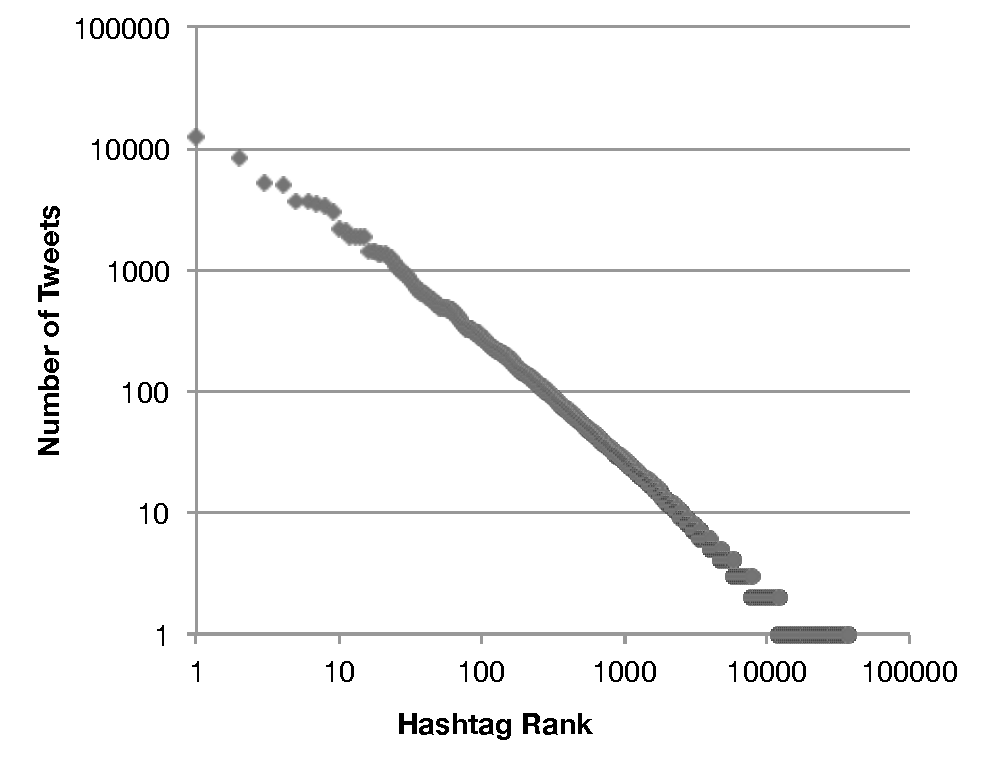
\includegraphics[scale=.5, viewport= 0cm 0cm 16.6cm 12.9cm]{hash-tag-dist.pdf}
\caption{2009 Twitter Hash Tag distribution on a log-log scale.
\label{fig:hash-dist}
}
\end{center}
\end{figure}

The power log scale shows us that there is a large spectrum of subscriber anonymity that can be taken advantage of. Colliding with popular tags gives you plausible deniability as there are relatively few tags dominating the space at a given time, and thus appear as legitimate interests. If there were a more even distribution of tags, then someone observing you following a particular tag would have less incentive to ignore suspicion that your activities might be objectionable to them. \hl{can we get a statistic on what the average number of tags someone follows is?}

\subsection{Collider}

In order to explore the feasibility of steering a particular Plain Tag to collide with an existing Short Tag, we built a collider tool. The tool takes in a Short Tag substring, \textit{T}, a prefix string, \textit{S}, a suffix length, \textit{L}, an alphabet 
\textit{A}. The collider finds the concatenations of \textit{S} and strings of length \textit{L} from \textit{A*} such that the truncated hash of the resultant string matches \textit{T}.

It has two modes of operation. In the default mode, he user specifies some number of tags to return that collide. The collider begins its scan at a random point in the search space and continues scanning until the requested number of tags are found. The second mode scans the entire search space, and therefore returns all matching tags for a given prefix and suffix length.

The search space, then, is of size $|A|^L$. If we wanted to match byte strings, $|A| = 256$, however, we decided to restrict the alphabet to alphanumeric characters due to Twitter's understanding of characters and not bytes, yielding $|A| = 62$. Additionally, the search space can be explored in parallel, giving the Collider executing on a system with \textit{P} processing units, a runtime of $O(\frac{62^L}{P})$.


\begin{figure}
\begin{center}
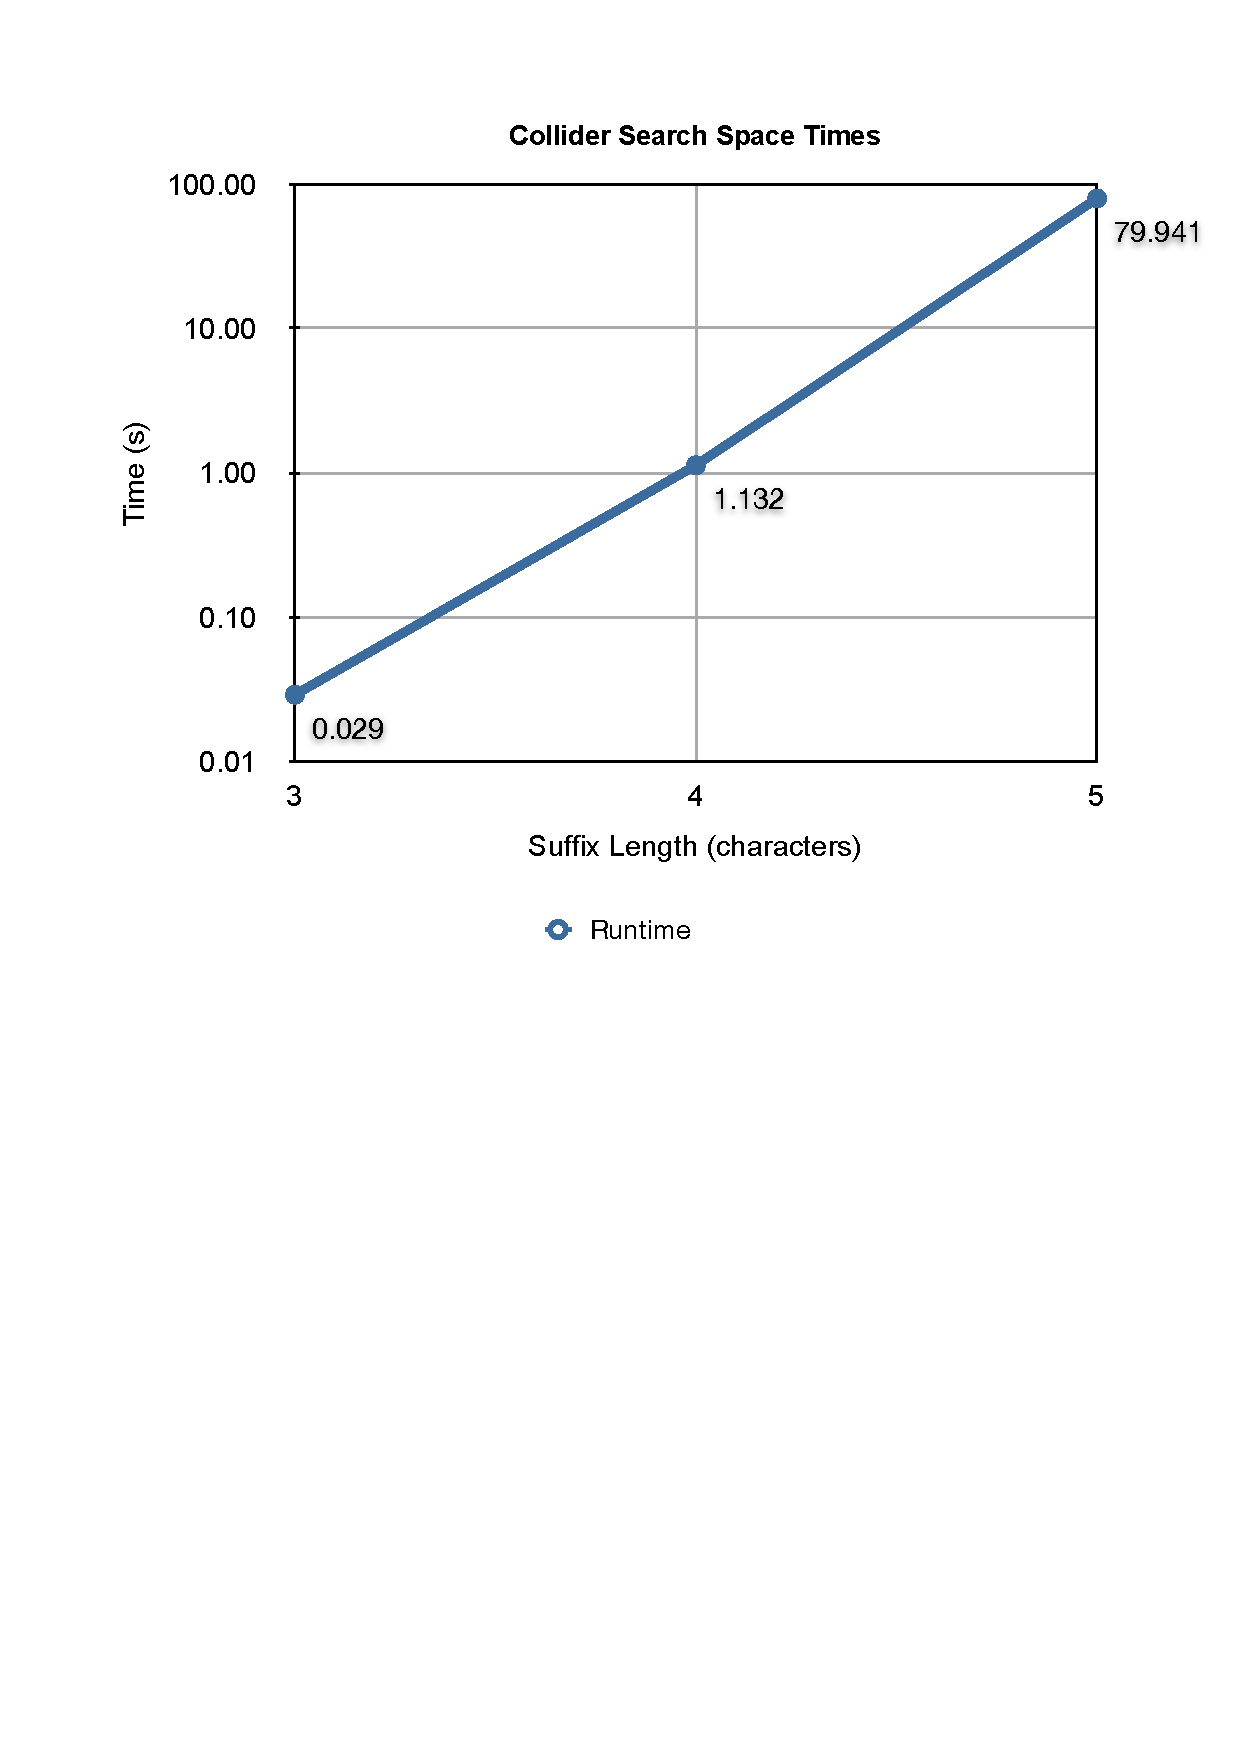
\includegraphics[scale=.5, viewport=0cm 0cm 16.6cm 13.6cm]{collider-times.pdf}
\caption{Runtime for the Collider to search the exploration spaces of sizes $62^3$, $62^4$, $62^5$ on dual quad-core Intel i5 processors.
\label{fig:collider-times}
}
\end{center}
\end{figure}

\begin{figure}
\begin{center}
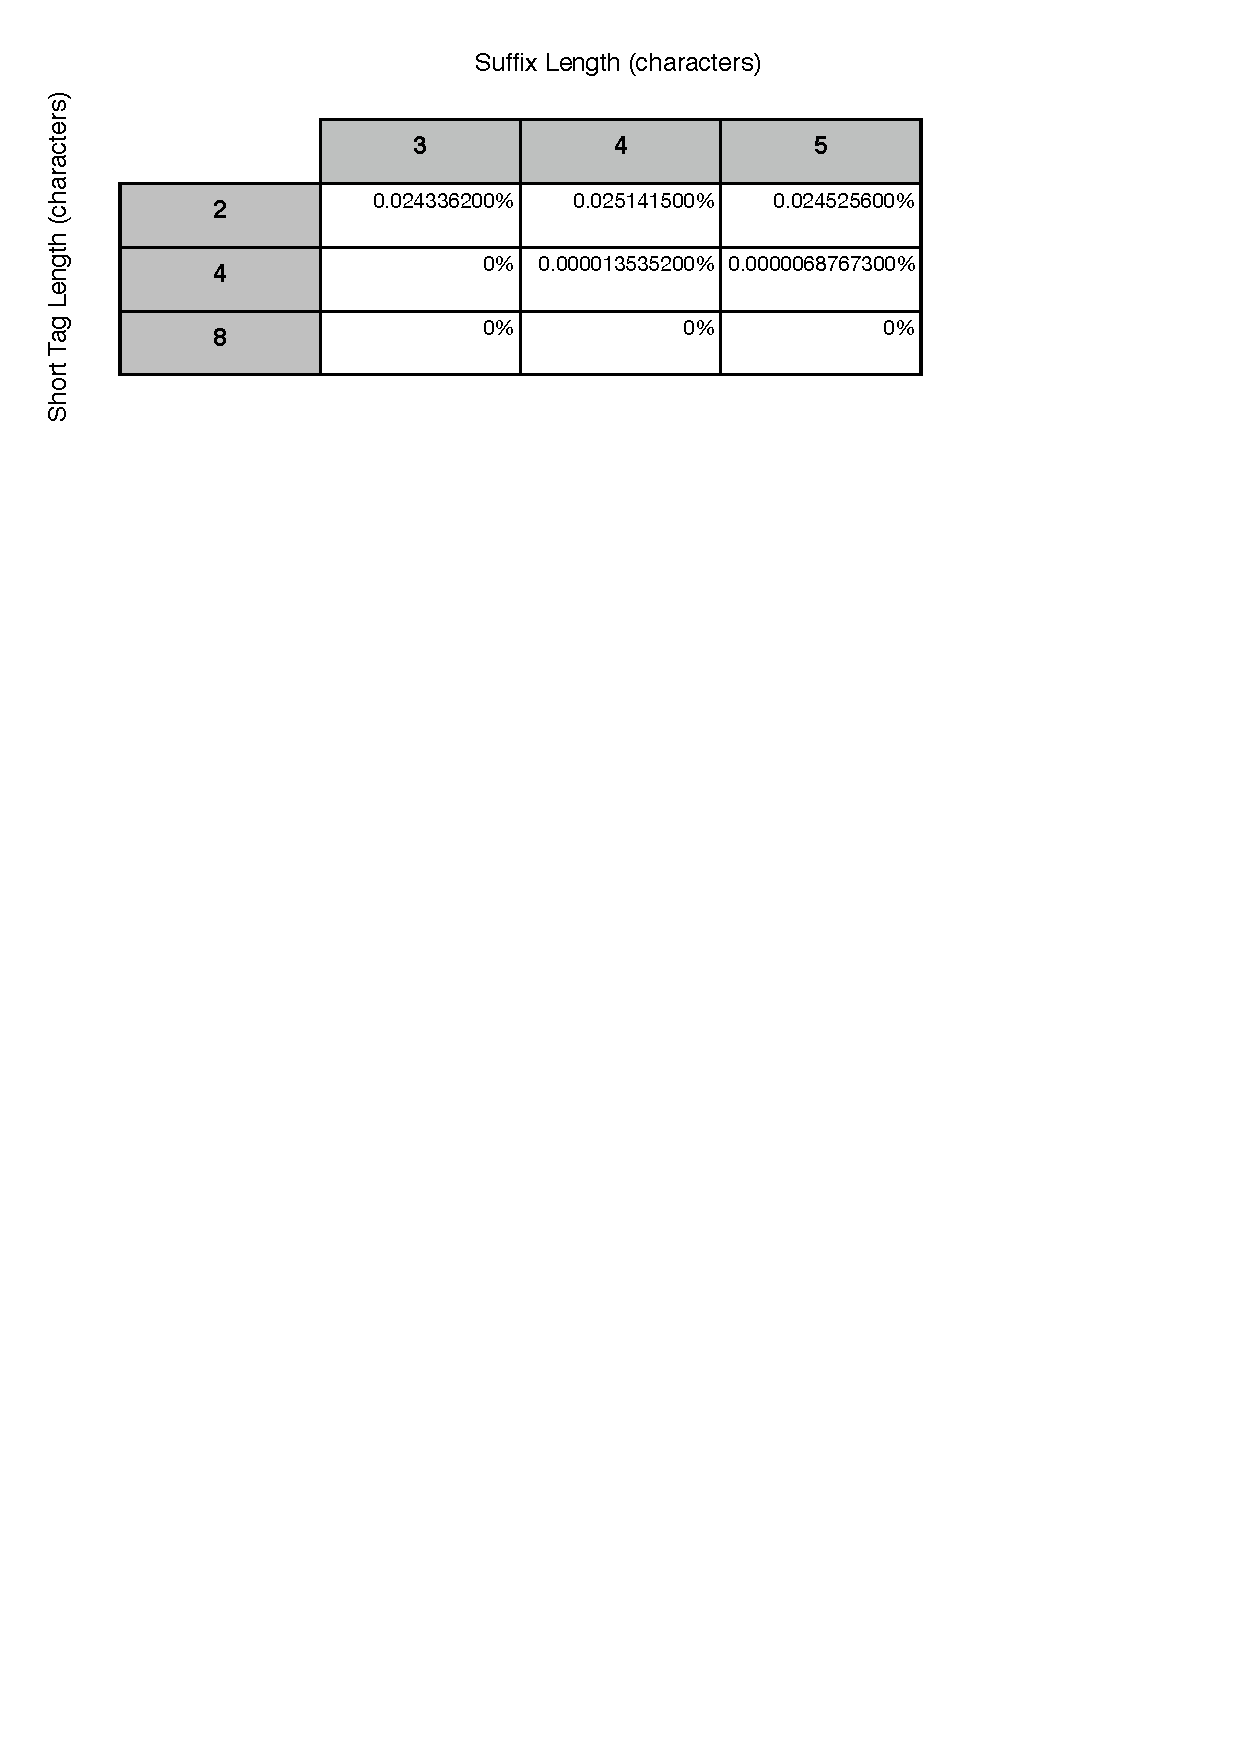
\includegraphics[scale=.5, viewport=0cm 0cm 16.5cm 7.5cm]{collider-hits.pdf}
\caption{Percent of search space that returned hits for an entered Short Tag, with a Prefix of `rice', and given Suffix Length. Length 2 prefix was `Ch', 4 was `Char', and 8 was `CharlieS'.
\label{fig:collider-hits}
}
\end{center}
\end{figure}

As expected, the runtime in Figure \ref{fig:collider-times} scales exponentially with \textit{L}, which in turn it becomes quickly infeasible for a single machine to do an exhaustive search of spaces where the suffix length is greater than 6.

Provided an attacker knows a particular group's prefix and the alphabet out of which they are generating the suffix, the embarrassingly parallel nature lends itself to brute force attacks. If we consider the adversary to be a government for example, it would be fair to assume they have thousands of machines at their disposal for such an attack. It becomes important, then for a user to pick a Plain Tag outside reasonable brute forcing bounds. 

\hl{should the `rememberable' limit discussion go here? or should this paragraph be moved out to discussion?}

Another concern is how easy it is to collide with another tag. From Fig. \ref{fig:collider-hits}, we find that beyond 4 characters, it was impossible to find collisions within easily searchable spaces (suffix sizes < 6). 

The results of these experiments place some limits on what choices a user can make currently regarding anonymity. You can only collide with up to 4 characters in a tag before the search space becomes such that any guarantee of collision is trivially small. Furthermore, $62^6$ is the upper bound on the search space for what a single computer can reasonably calculate a suffix to enable a collision with. Adding one more character to the suffix sends the computation into the span of days on a modern computer at time of writing.

However, we also show that tag collision is possible, there are certainly tunable degrees of anonymity thanks to the apparent power-log distribution of twitter tags already, and finding such a collision is feasibly done on a personal computer. \hl{What more to say here?}

\subsection{Performance}

In this experiment we wanted to see how well the encryption engine performed. In March 2011, Twitter stated that the site receives 140 million tweets per day or 1620 tweets per second on average (http://blog.twitter.com/2011/03/numbers.html). They also said that the maximum tweets per second ever was 6939. These numbers act as rough upper bounds to the number of Hoots per second the system would need to keep up with. In all likelihood, the number of encrypted messages posted would be drastically smaller than regular messages.

The benchmarks in Table \ref{tab:hps} were run on a 1.86GHz Intel Core 2 Duo, 4GB Ram, Macbook Air using Base64 encoding.


\begin{table}
\caption{Average Hoots Per Second for Encryption and Decryption
\label{tab:hps}
}
\begin{center}
    \begin{tabular}{ l  l }
	\hline
	Action & Average Hoots per second \\ \hline
	Encryption & 3614.531 \\
	Decryption & 15587.328 \\ \hline
    \end{tabular}
\end{center}
\end{table}


\hl{computation is negligible. one computer can do it, twittr has more than 1 comp. bandwidth is multiplied by more. more tweets per group. fundamentaly, twitter has to pay this for receiver anonymity. inherent to our scheme. Quantify how much. twitter's bandwitdh bill would go up and they aren't already making money. Cite sandler. people on average send 100 messages and have 100 followers. we dont know how big the groups, we can know how many poeple post, can't know how many listen. After incedient, lots of \#NotAFactualStatement. no idea how many actually listen. Many people could post w/o listening and viceversa. We could treat the numbers as equivelent but that's probbably not a factual statement.Cite: http://www.politico.com/news/stories/0411/53214.html}

Given these numbers, a Twitter server could easily encrypt the entire Twitter feed as the messages were posted. To handle peak usage like the 6939 tweets per second Twitter observed, many optimizations could be made, the simplest being to add a couple computers to help with the load. Our experiment shows that the Hoot protocol does not have significant overhead during encryption or decryption, so it can be adopted with little engineering effort.

It is interesting to note that the decryption rate is important to a client, since a client will be searching tweets trying to identify and decrypt potential Hoots. A client may not trust Twitter to do the decryption since that involves sharing the Plain Tag with Twitter, so a client would decrypt the message on their machine. Almost every client will not have a datacenter of computers for decryption, but our  process can decrypt Hoots almost five times faster than it encrypts them. A client, even with limited computing power, can easily keep up with the Twitter feed.

\hl{Should experiments have a wrap up paragraph?}
\section{Discussion}

In this section, we discuss a variety of issues and future extensions of the Hoot design.

\subsection{Incremental Rollout}

\hl{
1. Can you incrementally roll it out
	- Service provided by twitter or yourself
2. 140 character limit
	- Twitter doesn't have to go too far to have all the metadata for encryption
	
	- How hard is it for twitter to do this. 
	- Reference message fitting into 140 char using unicode
	- Reference peak hps, and how our system holds up
}
\subsection{Adoption}	

The next question to ask after we have shown that rolling out the Hoot service is feasible would be whether Twitter would actually implement such a feature. Based on the nature of Twitter, we believe that Twitter would not add a secure messaging framework like Hoot. Twitter as a company needs to know what people are talking about, so it can provide relevant advertisement. Adding the Hoot infrastructure to Twitter would prevent Twitter from knowing the content of the messages, and so we believe the Hoot service will never be adopted. However, this need not prevent individuals from using the Hoot protocol over Twitter. As long as Twitter faithfully delivers tweets, users are free to run the Hoot encryption on their own machines over their messages and then post the output to Twitter. In fact, this method is more secure in that a user only has to trust their machine. If Twitter is responsible for encrypting a message, nothing is stopping them from keeping a copy of the plain text message. Paranoid users will always want to encrypt messages themselves, so Twitter adopting the Hoot protocol is unnecessary.
		
\subsection{Usability}

As described in the Cover Traffic section, a group can deliberately collide with a popular tag by concatenating an easily rememberable string of text with random letters or numbers. As Miller\cite{miller56} noted, people can remember  
7 +/- 2 unique packets of data, so as long as these collisions can be generated with a suffix in that range a user is likely to be able to remember it. We could further improve rememberability by restricting suffix values to only digits, and then generate a suffix of 7 or 10 digits, emulating a phone number. The main requirement is that a group should be able to have a unique shared secret that can deliberately collide with other tags while still being easy to remember and more importantly easy to transfer. Since our proposal does not deal with key transfer, we assume our key communication is done through whisper channels and thus must be short and memorizable for simple transfer. We have found that a collision can be found with only appending 3-6 characters to a prefix, so deliberate collisions can both be found and transferred without much effort.

\hl{
-- Entropy 7+-2
-- Deliberate posting crap (to hide your stuff).
-- Increases work factor (signal to noise)
-- Fairly strong attacker, but user who don't have ability for a lot of entropy
-- 70 bits is enough compared to the weakness of everything else
}
\subsection{Alternate Backends}

Even though our protocol was designed with Twitter in mind, it is extensible to other systems and platforms. The Hoot protocol describes a secure way to transfer short messages (with short encryption overhead) across a publicly available network completely openly. Twitter is a great example of this environment but not the only one. Hoot could interact, for example, with a Distributed Hash Table system (DHT) like CHORD or Pastry. Importantly, Hoot can interface with both centralized systems like Twitter or Buzz or decentralized systems. As long as the platform's content is publicly searchable, the Hoot protocol allows secure transmission to anonymous group followers.

\hl{Discuss how we can make it harder for an attacker. Maybe hashing 1000 times...}
\section{Conclusions}

To provide censorship resistance and anonymity for groups wishing to communicate over a microblogging service like Twitter, we proposed \hoot. Hoots are private messages that are publicly posted but tagged with an identifier, allowing interested parties to efficiently find and decrypt them. By allowing many hash tags to collide with the same identifier, we protect recipient anonymity and use unrelated traffic as cover traffic. We found that \hoot can be added to a service like Twitter with little additional computational resources and reasonable additional bandwidth costs. We showed that users can have a experience that's virtually identical to a standard Twitter user, yet with radically better privacy. We also showed how it would be straightforward for Twitter to adopt \hoot and deploy it via web interfaces or via custom clients.


\bibliographystyle{abbrv}
\bibliography{hoot}

\balance

\end{document}
